%\documentclass[11pt]{report}
%\linespread{1.3} %1.3 for one and a half spacing, 1.6 for double
%\usepackage{amsmath, amsthm, amssymb, float, graphicx, caption, subcaption, cite, braket, url,color}
%%\usepackage[nohug,heads=vee]{diagrams}
%%\diagramstyle[labelstyle=\scriptstyle]
%%\graphicspath{{./Figures/}}
%\usepackage[margin=2.5cm]{geometry}
%%\title{Title}
%%\author{Chrysoula Vlachou}
%%\date{}
%\newtheorem{lemma}{Lemma}
%\newtheorem{theorem}{Theorem}
%\newtheorem{proposition}{Proposition}
%
%\newtheorem{definition}{Definition}
%\newcommand{\N}{\mathbb N}
%\newcommand{\R}{\mathbb R}
%\newcommand{\C}{\mathbb C}
%\newcommand{\Hilb}{\mathcal H}
%\newcommand{\HRule}{\rule{\linewidth}{0.5mm}}
%\newcommand{\mmobh}{\textlatin{M\"ob}(\mathbb{H})}
%\newcommand{\areah}{\textlatin{area}_{\mathbb{H}}}
%\newcommand{\dth}{d_{\mathbb{H}}}
%\newcommand{\tdth}{$d_{\mathbb{H}}$ }
%\def\h{\mathbb H}
%\DeclareMathOperator{\tr}{Tr}
%\def\I{\hat I}
%\def\ds{\displaystyle}
%\def\ppmod{\!\!\!\!\!\pmod}
%\newcommand{\q}[1]{\vec{#1}\cdot\vec{\sigma}}
%\usepackage{mathrsfs}
%
%
%\newcommand{\innerproduct}[2]{\langle #1 | #2 \rangle}
%\def\mobh{\textlatin{M\"ob}({\mathbb H})}
%
%
%
%\begin{document}
\chapter{Phase transitions at finite temperatures of topological systems out of equilibrium}

 



In this chapter, we investigate the existence of finite-temperature PTs in topological systems out of equilibrium. As mentioned in the Introduction, recently, there have been proposed two different approaches to DPTs, which give opposite predictions. Our goal is to compare and contrast these two approaches and clarify which is the one that better captures the many-body nature of these systems.
This chapter is organised as follows: in Section~\ref{Sec: DQPTs and Susceptibilities}, after a brief introduction to the study of DQPTs in the case of pure states, we proceed by analytically deriving the two different finite-temperature generalisations of the LE (fidelity LE and interferometric LE) and the associated susceptibilities, which give opposite predictions about the fate of DQPTs in the case of mixed states. Subsequently, we specialise this derivation in the case of two-band Hamiltonians, since the topological systems that we are interested in are described by such Hamiltonians. Based on the analysis of the two different dynamical susceptibilities, we compare the two approaches to DPTs, analyse the reasons for their different predictions and argue that the fidelity LE approach is more suitable in the case of realistic many-body systems.  
In Section~\ref{sec:num.results}, we present quantitative results for the fidelity-induced first time derivative of the rate function in the case of the 1D SSH model~\cite{su:sch:hee:79} of a TI and the 2D Massive Dirac (MD) model of a Chern insulator~\cite{qi:hug:zha:08}. Finally, in the last section we summarise our results and present our conclusions.\\  
\vfill

\begin{center}
 *The work presented in this chapter corresponds to the work published in~\cite{mer:vla:pau:vie:viy:18}.
\end{center}

\newpage


\section{Dynamical (quantum) phase transitions and the associated susceptibilities}
\label{Sec: DQPTs and Susceptibilities}
The authors in~\cite{hey:pol:keh:13} introduce the concept of DQPTs and illustrate their properties in the case of the transverse-field Ising model. They observe a similarity between the partition function of a quantum system in equilibrium, $Z(\beta)=\tr(e^{-\beta H})$, and the overlap amplitude of some time-evolved initial quantum state $\ket{\psi_i}$ with itself, $G(t)=\langle\psi_i|e^{-iHt}|\psi_i\rangle$. During a temperature-driven PT, the abrupt change of the properties of the system is indicated by the non-analyticity of the free energy density $f(\beta)=-\lim_{N\to\infty}\frac{1}{N}\ln Z(\beta)$ at the critical temperature ($N$ being the number of degrees of freedom). It is then possible to establish an analogy with the case of the real-time evolution of a quantum system out of equilibrium, by considering the rate function 
\begin{equation}
\label{eq:rate}
g(t)=-\frac{1}{N}\log |G(t)|^2,
\end{equation} 
where $|G(t)|^2$ is a mixed-state LE, as we detail below. The rate function $g(t)$ may exhibit non-analyticities at some critical times $t_c$, after a quantum quench. 


\subsection{DQPTs for pure states}
\label{Subsec: DQPT for pure states}

At zero temperature, the LE $G(t)$ from Equation~\eqref{eq:rate} between the ground state for $\lambda=\lambda_i\in M$ and the evolved state with respect to the Hamiltonian for $\lambda=\lambda_f\in M$ is given by the fidelity between the two states
\begin{eqnarray}
\mathcal{F}(t;\lambda_{f},\lambda_i)\equiv |\bra{\psi(\lambda_i)}e^{-it H(\lambda_f)}\ket{\psi(\lambda_i)}|.
\label{Eq: zero temperature fidelity}
\end{eqnarray}
For $\lambda_i=\lambda_f$, the fidelity is trivial, since the system remains in the same state. Fixing $\lambda_i\equiv \lambda$ and $\lambda_{f} = \lambda + \delta\lambda$, with $\delta\lambda<<1$, in the $t\rightarrow\infty$ limit Equation~\eqref{Eq: zero temperature fidelity} is nothing but the familiar $S$-matrix with an unperturbed Hamiltonian $H(\lambda)$ and an interaction Hamiltonian $V(\lambda)$, which is approximated by
\begin{eqnarray}
V(\lambda)\equiv H(\lambda_f)-H(\lambda)\approx\frac{\partial H}{\partial \lambda^{a}}(\lambda)\delta \lambda^a.
\label{Eq:2}
\end{eqnarray}
After applying standard perturbation theory techniques (see Appendix B),
 we obtain
\begin{eqnarray}
\mathcal{F}(t;\lambda_f,\lambda)\approx 1 -\chi_{ab}(t;\lambda)\delta \lambda^a \delta \lambda^b,
\end{eqnarray}
where the dynamical susceptibility $\chi_{ab}(t;\lambda)$ is given by
\begin{small}
\begin{eqnarray}
&\chi_{ab}(t;\lambda)=\nonumber \\
&\int_{0}^{t}\int_{0}^{t} dt_2dt_1 \left(\frac{1}{2}\langle \{V_{a}(t_2),V_{b}(t_1)\} \rangle-\langle V_{a}(t_2)\rangle \langle V_{b}(t_1) \rangle\right),
\label{Eq: zero temperature susceptibility}
\end{eqnarray}
\end{small}with $V_{a}(t,\lambda)=e^{it H(\lambda)}\partial H/\partial \lambda^{a}(\lambda)e^{-it H(\lambda)}$ and $\langle \ast\rangle=\bra{\psi(\lambda)}\ast\ket{\psi(\lambda)}$. The family of symmetric tensors $\{ds^2(t)=\chi_{ab}(t,\lambda)d\lambda^a d\lambda^b\}_{t\in \mathbb{R}}$ defines a family of metrics in the manifold $M$, which can be seen as pullback metrics of the Bures metric (Fubini-Study metric) in the manifold of pure states~\cite{chr:jam:12}. Specifically, at time $t$, the pullback is given by the map $\Phi_t: \lambda_f \mapsto e^{-it H(\lambda_f)}\ket{\psi(\lambda)}\bra{\psi(\lambda)}e^{i t H(\lambda_f)}$, evaluated at $\lambda_f=\lambda$.
 
\subsection{Generalisations at finite temperatures}
\label{Subsec: DQPT for pure states}


The generalisation of DQPTs to mixed states is not unique. There are several ways to construct a LE for a general density matrix. In what follows, we derive two finite-temperature generalisations, such that they have the same zero-temperature limit. \\
\subsubsection{Fidelity Loschmidt Echo at $T>0$}


First, we introduce the {\em fidelity LE} between the state $\rho(\beta;\lambda_i)=e^{-\beta H(\lambda_i)}/\tr\{e^{-\beta H(\lambda_i)}\}$ and the one evolved by the unitary operator $e^{-it H(\lambda_f)}$ as
\begin{eqnarray}
\!\!\!\!\!\!\mathcal{F}(t,\beta;\lambda_i,\lambda_f)\!=\!F(\rho(\beta;\lambda_i),e^{-it H(\lambda_f)}\rho(\beta;\lambda_i)e^{itH(\lambda_f)}),
\label{eq:fid}
\end{eqnarray}
where $F(\rho,\sigma)=\tr\{\sqrt{\sqrt{\rho}\sigma\sqrt{\rho}}\}$ is the quantum fidelity between arbitrary mixed states $\rho$ and $\sigma$. For $\lambda_f$ close to $\lambda_i=\lambda$, we can write
\begin{eqnarray}
\mathcal{F}(t,\beta ;\lambda_f,\lambda)\approx 1 -\chi_{ab}(t,\beta ;\lambda)\delta \lambda^a \delta \lambda^b,
\end{eqnarray}
with $\chi_{ab}(t,\beta,\lambda)$ being the \emph{Dynamical Fidelity Susceptibility} (DFS). Notice that $$\lim_{\beta\to\infty}\chi_{ab}(t,\beta;\lambda)=\chi_{ab}(t;\lambda),$$ where $\chi_{ab}(t;\lambda)$ is given by Equation~\eqref{Eq: zero temperature susceptibility}. At time $t$ and inverse temperature $\beta$, we have a map $\Phi_{(t,\beta)}: \lambda_f\mapsto e^{-i tH (\lambda_f)} \rho(\beta;\lambda) e^{it H(\lambda_f)}$. The $2$-parameter family of metrics defined by $ds^2(\beta,t)=\chi_{ab}(t,\beta;\lambda)d\lambda^{a}d\lambda^b$ is the pullback by $\Phi_{(t,\beta)}$ of the Bures metric on the manifold of full-rank density operators, evaluated at $\lambda_f=\lambda$ (see Appendix B).

The fidelity LE is closely related to the Uhlmann connection: $F(\rho_1,\rho_2)$ equals the overlap between purifications $W_1$ and $W_2$, $\langle W_1,W_2\rangle=\tr \left\{W_1^\dagger W_2\right\}$, satisfying discrete parallel transport condition (see, for instance,~\cite{uhl:11}). 


\subsubsection{Interferometric Loschmidt Echo at $T>0$}

Here, we consider an alternative generalisation of the LE for mixed states [$G(t)$ from Equation~\eqref{eq:rate}]. In particular, we define the {\em interferometric LE} as
\begin{eqnarray}
\mathcal{L}(t,\beta ;\lambda_{f},\lambda_i)=\left|\frac{\tr\left\{e^{-\beta H(\lambda_i)} e^{i tH(\lambda_i)}e^{-i t H(\lambda_f)}\right\}}{\tr \left\{e^{-\beta H(\lambda_i)}\right\}}\right|.
\end{eqnarray}
The $e^{it H(\lambda_i)}$ factor does not appear at zero temperature, since it just gives a phase which is canceled by taking the absolute value.  This differs from previous treatments in the literature~\cite{bud:hey:16} (see Section~5.5.4 of~\cite{chr:jam:12}, where the variation of the interferometric phase, $\tr\{\rho_0 e^{-it H}\}$, exposes this structure). However, it is convenient to introduce it in order to have the usual form of the perturbation expansion, as will become clear later.

For $\lambda_f$ close to $\lambda_i=\lambda$, we get
\begin{eqnarray}
\mathcal{L}(t,\beta ;\lambda_f,\lambda)\approx \left|\frac{\tr\left\{e^{-\beta H(\lambda)} T e^{-i \int_{0}^{t} dt' V_{a}(t,\lambda) \delta \lambda^a}\right\}}{\tr \left\{e^{-\beta H(\lambda)}\right\}}\right|,
\end{eqnarray}
so that the perturbation expansion goes as in Equation~\eqref{Eq: zero temperature susceptibility}, yielding
\begin{eqnarray}
\mathcal{L}(t,\beta ;\lambda_f,\lambda)\approx 1 -\tilde\chi_{ab}(t,\beta ;\lambda)\delta \lambda^a \delta \lambda^b,
\end{eqnarray}
with the dynamical susceptibility given by
\begin{small}
\begin{equation}
\tilde{\chi}_{ab}(t,\beta;\lambda)=
\int_{0}^{t}\int_{0}^{t} dt_2dt_1  \left(\frac{1}{2}\langle \{V_{a}(t_2),V_{b}(t_1)\} \rangle-\langle V_{a}(t_2)\rangle \langle V_{b}(t_1) \rangle\right),
\label{Eq: finite temperature interferometric susceptibility}
\end{equation}
\end{small}where $\langle \ast\rangle=\tr\{e^{-\beta H(\lambda)}\ast\}/\tr\{e^{-\beta H(\lambda)}\}$. Notice that Equations~\eqref{Eq: finite temperature interferometric susceptibility} and~\eqref{Eq: zero temperature susceptibility} are formally the same with the average over the ground state replaced by the thermal average. This justifies the extra $e^{it H(\lambda_i)}$ factor. Since this susceptibility comes from the interferometric LE, we call it \emph{Dynamical  Interferometric Susceptibility} (DIS). The quantity $ds^2(\beta,t)=\tilde{\chi}_{ab}(t,\beta;\lambda)d\lambda^ad\lambda^b$ defines a $2$-parameter family of metrics over the manifold $M$, except that they cannot be seen as pullbacks of metrics on the manifold of density operators with full rank. However, it can be interpreted as the pullback by a map from $M$ to the unitary group associated with the Hilbert space of a particular Riemannian metric. For a detailed analysis, see Appendix B. Note that this version of the LE is related to the interferometric geometric phase introduced by Sj\"{o}qvist \emph{ et. al}~\cite{sjo:pat:eke:ana:eri:oi:ved:00,ton:sjo:kwe:oh}. \\

\subsection{Two-band systems}

Many representative examples of TIs and TSCs can be described by effective two-band Hamiltonians. Therefore, we derive closed expressions of the previously introduced dynamical susceptibilities for topological systems within this class. 

The general form of such Hamiltonians is $\{H(\lambda)=\vec{x}(\lambda)\cdot \vec\sigma:\lambda \in M\}$, where $\vec{\sigma} $  is the Pauli vector. The interaction Hamiltonian $V(\lambda)$, introduced in Equation~\eqref{Eq: zero temperature fidelity}, casts the form
\begin{equation*}
V(\lambda)\approx \left(\frac{\partial \vec{x}}{\partial\lambda^a}\cdot \vec{\sigma}\right) \delta \lambda^a.
\end{equation*} 
It is convenient to decompose $\partial\vec{x}/\partial \lambda^a$ into one component perpendicular to $\vec{x}$ and one parallel to it:
\begin{equation*}
\frac{\partial \vec{x}}{\partial\lambda^a}=\left(\frac{\partial \vec{x}}{\partial\lambda^a}\right)^{\perp}+ \left(\frac{\partial \vec{x}}{\partial\lambda^a}\right)^{\parallel}=\vec{t}_{a}+\vec{n}_a.
\end{equation*}
The first term is tangent, in $\mathbb{R}^3$, at $\vec{x}(\lambda)$, to a sphere of constant radius $r=|\vec{x}(\lambda)|$. Hence, this kind of perturbations does not change the spectrum of $H$, only its eigenbasis. The second term is a variation of the length of $\vec{x}$ and hence, it changes the spectrum of $H$, while keeping the eigenbasis fixed. The DFS and the DIS are given by (for the details of the derivation, see Appendix B)
\begin{small}
\begin{eqnarray}
\label{Eq: DFS}
\chi_{ab}&=&\tanh^2(\beta |\vec{x}(\lambda)|)\frac{\sin^2(|\vec{x}(\lambda)|t)}{|\vec{x}(\lambda)|^2}\vec{t}_a\!\!\cdot\!\vec{t}_b \\
\label{Eq: DIS}
\tilde{\chi}_{ab}\!&=&\!\frac{\sin^2(|\vec{x}(\lambda)|t)}{|\vec{x}(\lambda)|^2}\vec{t}_a\!\!\cdot\!\vec{t}_b\!+\!t^2(1\!\!-\!\!\tanh^2(\beta |\vec{x}(\lambda)|))\vec{n}_a\!\!\!\cdot\!\vec{n}_b.
\end{eqnarray}
\end{small}

While the DIS from Equation~\eqref{Eq: DIS} depends on the variation of both the spectrum and the eigenbasis of the Hamiltonian, the DFS from Equation~\eqref{Eq: DFS} depends only on the variations which preserve the spectrum, i.e., changes in the eigenbasis. This is quite remarkable, since in general the fidelity between two quantum states, being their distinguishability measure, does depend on both the variations of the spectrum and the eigenbasis. In our particular case of a quenched system, the eigenvalues are preserved (see Equation~\eqref{eq:fid}), as the system is subject to a unitary evolution. The tangential components of both susceptibilities are modulated by the function $\sin ^2 (Et)/ E^2$, where $E$ is the gap. This captures the \emph{Fisher zeros}, i.e., the zeros of the (dynamical) partition function which here is given by the fidelity $\mathcal F$ from Equation~\eqref{eq:fid}, see~\cite{yan:lee:52,lee:yan:52, fis:65}. Observe that whenever $t=(2n+1)\pi/2E$, $n\in\mathbb{Z}$, this factor is maximal and hence, both LEs decrease abruptly.
The difference between the two susceptibilities is given by
\begin{equation*}
\tilde{\chi}_{ab}-\chi_{ab}
=(1-\tanh^2(\beta|\vec{x}(\lambda)|))\left(\frac{\sin^2(|\vec{x}(\lambda)|t)}{|\vec{x}(\lambda)|^2}\vec{t}_a\cdot \vec{t}_{b} +t^2\vec{n}_a\cdot \vec{n}_b\right).
\end{equation*}
The quantity $(1-\tanh^2(\beta E))$ is nothing but the static susceptibility, see~\cite{pat:96}. Therefore, the difference between DIS and DFS is modulated by the static susceptibility at finite temperature. 

\begin{figure}[h]
\begin{center}
    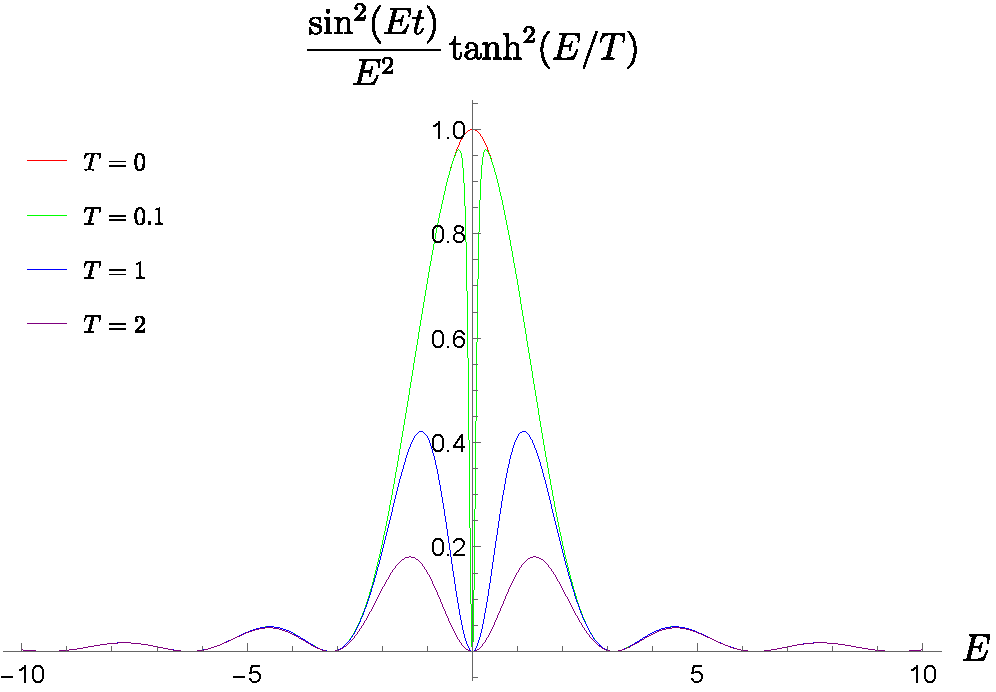
\includegraphics[scale=0.5]{susceptibility.pdf}
    \caption{The susceptibility modulating function for the tangential components at $t=1$.}
\end{center}
\label{fig:suscep}
\end{figure}


To illustrate the relationship between the two susceptibilities, in Figure~6.1 we plotted the modulating function for the tangential components of both. We observe that at zero temperature they coincide. As the temperature increases, in the case of the fidelity LE, the gap-vanishing points become less important. On the contrary, for the interferometric LE, the associated tangential part of the susceptibility does not depend on temperature, thus the gap-vanishing points remain prominent. The DFS from Equation~\eqref{Eq: DFS} thus predicts gradual smearing of critical behaviour, consistent with our results from the previous two chapters that showed the absence of PTs at finite temperatures in the static case. The DIS from Equation~\eqref{Eq: DIS} has a tangential term that is not coupled to the temperature, persisting at higher temperatures and giving rise to abrupt changes in the finite-temperature system's behaviour. This is also consistent with previous studies in the literature, where DPTs were found even at finite temperatures~\cite{hey:bud:17, bah:ban:dut:17}. Additionally, the interferometric LE depends on the normal components of the variation of $\vec{x}$. In other words, the finite-temperature PTs inferred by the behaviour of the interferometric LE occur due to the change of the parameters of the Hamiltonian and not due to temperature. 


\subsection{Comparing the two approaches}

The above analysis of the two dynamical susceptibilities (metrics) reflects the essential difference between the two distinguishability measures, one based on the fidelity, the other on  interferometric experiments. From the quantum information theoretical point of view, the two quantities can be interpreted as distances between \emph{states}, or between \emph{processes}, respectively. The Hamiltonian evaluated at a certain point of parameter space $M$ defines the macroscopic phase. Associated to it we have thermal states and unitary processes. The fidelity LE is obtained from the Bures distance between a thermal state $\rho_1$ in phase $1$ and the one obtained by unitarily evolving this state, $\rho_2 = U_2\rho_1 U_2^{\dagger}$, with $U_2$ associated to phase $2$.  Given a thermal state $\rho_1$ prepared in phase $1$, the interferometric LE is obtained from the distance between two unitary processes $U_1$ and $U_2$ (defined modulo a phase factor), associated to phases $1$ and $2$.  

The quantum fidelity between two states is in fact the classical fidelity between the probability distributions obtained by performing an optimal measurement on them. Measuring an observable $M$ on the two states $\rho_1$ and $\rho_2$, one obtains the probability distributions $\{p_1(i)\}$ and $\{p_2(i)\}$, respectively. The quantum fidelity $F_Q$ between the two states $\rho_1$ and $\rho_2$ is bounded by the classical fidelity $F_C$ between the probability distributions $\{p_1(i)\}$ and $\{p_2(i)\}$, $F_Q (\rho_1,\rho_2) = \mbox{Tr}\sqrt{\sqrt{\rho_1}\rho_2\sqrt{\rho_1}} \leq \sum_i \sqrt{p_1(i)p_2(i) = F_c (p_1(i),p_2(i))}$, such that the equality is obtained by measuring an {\em optimal observable}, given by $M_{\text{op}} = \rho_1^{-1/2}\sqrt{\sqrt{\rho_1}\rho_2\sqrt{\rho_1}} \rho_1^{-1/2}$ (note that optimal observable is not unique). For that reason, one can argue that the fidelity is capturing all order parameters (i.e., measurements) through its optimal observables $M_{\text{op}}$. Fidelity-induced distances, the {\em Bures distance} $D_B(\rho_1,\rho_2) = \sqrt{2(1-F_Q(\rho_1,\rho_2))}$, the {\em sine distance} $D_S(\rho_1,\rho_2) = \sqrt{1-F_Q^2(\rho_1,\rho_2)}$ and the {\em F-distance} $D_F(\rho_1,\rho_2) = 1-F_Q(\rho_1,\rho_2)$ satisfy the following set of inequalities
\begin{equation*}
	 D_F(\rho_1,\rho_2) \leq D_T(\rho_1,\rho_2) \leq D_S(\rho_1,\rho_2) \leq D_B(\rho_1,\rho_2),
\end{equation*}
where the {\em trace distance} is given by $D_T(\rho_1,\rho_2) = \frac{1}{2} \mbox{Tr}|\rho_1 - \rho_2|$. In other words, the fidelity-induced distances and the trace distance establish the same order on the space of quantum states. This is important, as the trace distance is giving the optimal value for the success probability in ambiguously discriminating in a {\em single shot-measurement} between two {\em a priori}equally probable states $\rho_1$ and $\rho_2$, given by the so-called Helstrom bound $P_H (\rho_1,\rho_2) = (1 + D_T (\rho_1,\rho_2))/2$~\cite{hel:76}.

On the other hand, the interferometric phase is based on some interferometric experiment to distinguish two states, $\rho_1 = \sum_i r_i \ket{i}\bra{i}$ and $\rho_2 = U_2 \rho_1 U_2^{\dagger}$: it measures how the intensities at the outputs of the interferometer are affected by applying $U_2$ to only one of its arms~\cite{sjo:pat:eke:ana:eri:oi:ved:00}. Therefore, to set up such an experiment, one does not need to know the state $\rho_1$ that enters the interferometer, as only the knowledge of $U_2$ is required. Note that this does not mean that the output intensities do not depend on the interferometric LE: indeed, the inner product $\langle U_1,U_2\rangle_{\rho_1}$ is defined with respect to the state $\rho_1$. This is a different type of experiment, not based on the observation of any physical property of a system. It is analogous to comparing two masses with weighing scales, which would show the same difference of $\Delta m = m_1 - m_2$, regardless of how large the two masses $m_1$ and $m_2$ are. For that reason, interferometric distinguishability is more sensitive than the fidelity (fidelity depends on more information, not only how much the two states are different, but in what aspects this difference is observable). Indeed,  the interferometric LE between $\rho_1$ and $\rho_2$ can be written as the overlap $L(\rho_1, \rho_2) = |\langle \rho_1|\rho_2\rangle|$ between the purifications $|\rho_1\rangle = \sum_i  \sqrt{r_i} |i\rangle|i\rangle$ and $|\rho_2\rangle=(U\otimes I)|\rho_1\rangle$. On the other hand, the fidelity satisfies $F(\rho_1, \rho_2) = \max_{|\psi\rangle,|\varphi\rangle} |\langle\psi|\varphi\rangle|$, where $|\psi\rangle$ and $|\varphi\rangle$ are purifications of $\rho_1$ and $\rho_2$, respectively, i.e., $L(\rho_1, \rho_2) \leq F(\rho_1, \rho_2)$. Moreover, what one does observe in interferometric experiments are the mentioned output intensities, i.e., one needs a number of identical systems prepared in the same state to obtain results in interferometric measurements. This additionally explains why interferometric LE is more sensible than the fidelity one, as the latter is based on the observations performed on single systems. The fact that interferometric LE is more sensitive than the fidelity LE is consistent with the result that the former is able to capture the changes of some of the system's features at finite temperatures (thus they predict DPTs), while the latter cannot.

In terms of experimental feasibility, the fidelity is more suitable for the study of many-body macroscopic systems and phenomena, while the interferometric measurements provide a more detailed information on genuinely quantum (microscopic) systems. Finally, interferometric experiments involve coherent superpositions of two states. Therefore, when applied to many-body systems, one would need to create genuine Schr\"{o}dinger cat-like states, which goes beyond the current, and any foreseeable, technology (and could possibly be forbidden by more fundamental laws of physics; see for example objective collapse theories~\cite{bas:loc:sat:sin:ulb:13}).  

\section{DPTs of topological insulators at finite temperatures}
\label{sec:num.results}
Our general study of two-band Hamiltonians showed that the fidelity-induced LE predicts a gradual smearing of DPTs with temperature. In order to further confirm this result, we study the fidelity LE for two concrete examples of TIs (the analogous study for the interferometric LE on concrete examples has already been performed, and is consistent with our findings~\cite{hey:bud:17,bah:ban:dut:17}). In particular, we present quantitative results obtained for the first derivative of the rate function, $dg/dt$, where $g(t)=-\frac{1}{N}\log \mathcal{F}$, and 
\begin{equation*}
\mathcal{F}(t,\beta;\lambda_i,\lambda_f)=F(\rho(\beta;\lambda_i),e^{-it H(\lambda_f)}\rho(\beta;\lambda_i)e^{itH(\lambda_f)}).
\end{equation*}

The fidelity $F$ is obtained by taking the product of the single-mode fidelities, each of  which has the form
\begin{footnotesize}
\begin{eqnarray*}
F(\rho(\beta;\lambda_i),e^{-it H(\lambda_f)}\rho(\beta;\lambda_i)e^{itH(\lambda_f)}) =\sqrt{\frac{1+\cosh^2(\beta E_i)+\sinh^2(\beta E_i)\left[\cos(2E_f t)+(1-\cos(2E_f t))(\vec{n}_i\cdot\vec{n}_f)^2)\right]}{2\cosh^2(\beta E_i)}},	
\end{eqnarray*}\end{footnotesize}with $H_a=E_a\vec{n}_a\cdot \vec{\sigma}$ and $a=i,f$. This expression can be obtained by using Equation~\eqref{eq:su(2)toso(3)} and the result found in Appendix A. The quantity $dg/dt$ is the figure of merit in the study of the DQPTs, therefore we present the respective results that confirm the previous study: the generalisation of the LE with respect to the fidelity shows the absence of finite-temperature DPTs.  The models of TIs that we consider are the SSH~\cite{su:sch:hee:79} and the MD~\cite{qi:hug:zha:08} model. 


\subsection{SSH model (1D)}
The SSH model was introduced in~\cite{su:sch:hee:79} to describe polyacetilene, and it was later found to describe diatomic polymers~\cite{ric:mel:82}. In momentum space, the Hamiltonian for this model is of the form $H(k,m)=\vec{x}(k,m)\cdot\vec{\sigma},$ with $m$ being the parameter that drives the static PT. The vector $\vec{x}(k,m)$ is given by:
\begin{equation*}
\vec{x}(k,m)=(m+\cos(k),\sin(k),0).
\end{equation*}

By varying $m$ we find two distinct topological regimes. For $m<m_c=1$ the system is in a non-trivial phase with winding number $1$, while for $m>m_c=1$ the system is in a topologically trivial phase with winding number $0$.

We consider both cases in which we go from a trivial to a topological phase and vice versa (Figures~6.2 and~6.3, respectively). We notice that non-analyticities of the first derivative appear at zero temperature, and they are smeared out for higher temperatures.

\begin{figure}[h]
\begin{center}
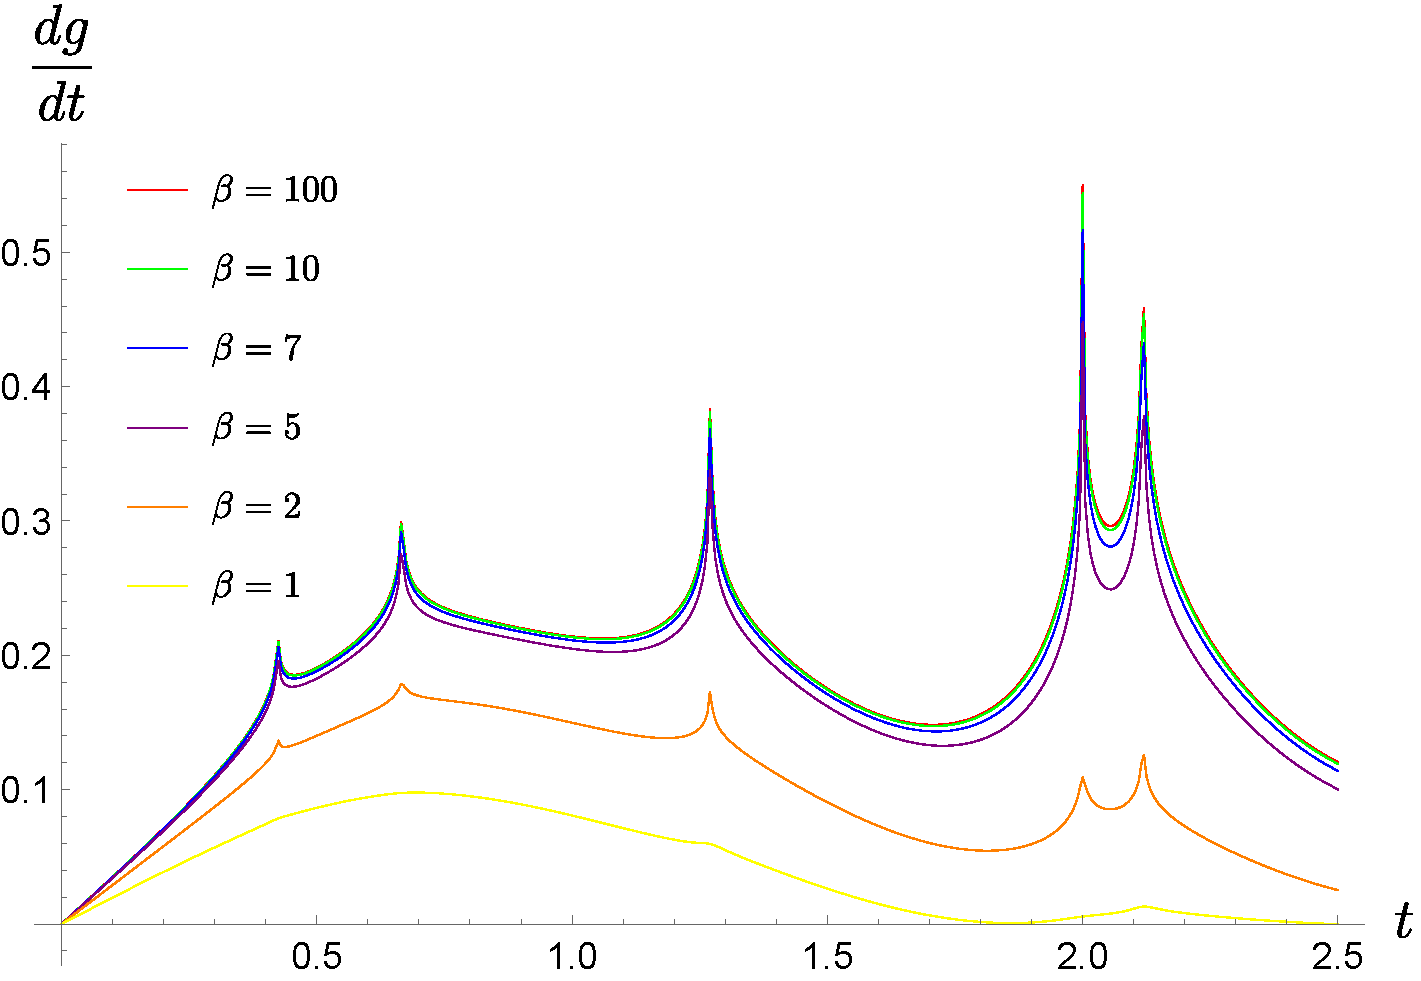
\includegraphics[scale=0.3]{SSH_trivial_to_topological.pdf}
\caption{We plot the time derivative of the rate function, $dg/dt$, as a function of time for different values of the inverse temperature $\beta=1/T$. We consider a quantum quench from a trivial phase $(m=1.2)$ to a topological phase $(m=0.8)$.}
\end{center}  
\label{fig:SSHtrivialtopological}
\end{figure}


\begin{figure}[h]
\begin{center}
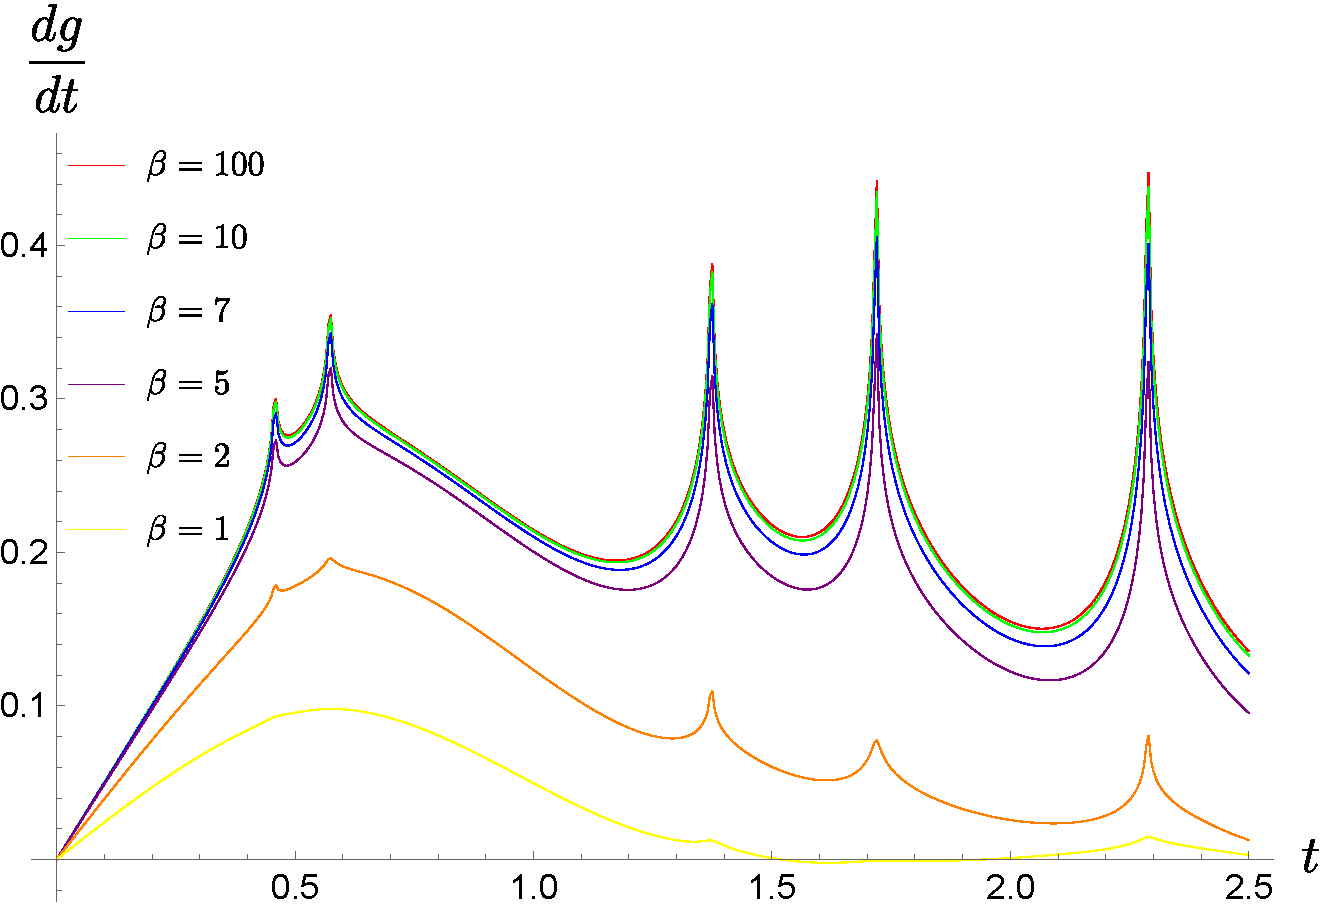
\includegraphics[scale=0.3]{SSH_topological_to_trivial.pdf}
    \caption{The time derivative of the rate function, $dg/dt$, as a function of time for different values of the inverse temperature. The quench is from a topological $(m=0.8)$ to a trivial phase $  (m=1.2)$.}
\end{center}
\label{fig:SSHtopologicaltrivial}
\end{figure}


\subsection{MD model (2D)}


The Massive Dirac model (MDM) captures the physics of a 2D Chern insulator~\cite{qi:hug:zha:08}, and features several different topologically distinct phases. In momentum space, the Hamiltonian for the MDM is of the form $H(\vec{k},m)=\vec{x}(\vec{k},m)\cdot\vec{\sigma},$ with $m$ being the parameter that drives the static PT. The vector $\vec{x}(\vec{k},m)$ is given by
\begin{equation*}
\vec{x}(\vec{k},m)=(\sin(k_x),\sin(k_y),m-\cos(k_x)-\cos(k_y)).
\end{equation*}
By varying $m$ we find four different topological regimes:

\begin{itemize}
\item For $-\infty<m<m_{c_1}=-2$ it is trivial (the Chern number is zero) -- Regime I
\item For $-2=m_{c_1}<m<m_{c_2}=0$ it is topological (the Chern number is $-1$) -- Regime II
\item For $0=m_{c_2}<m<m_{c_3}=2$ it is topological (the Chern number is $+1$) -- Regime III
\item For $2=m_{c_3}<m<\infty$ it is trivial (the Chern number is zero) -- Regime IV
\end{itemize}


In Figures~6.4,~6.5 and~6.6 we plot the first derivative of the rate function $g(t)$, as a function of time for different temperatures. We only consider quenches that traverse a single PT point. 

\begin{figure}[h]
\begin{center}
    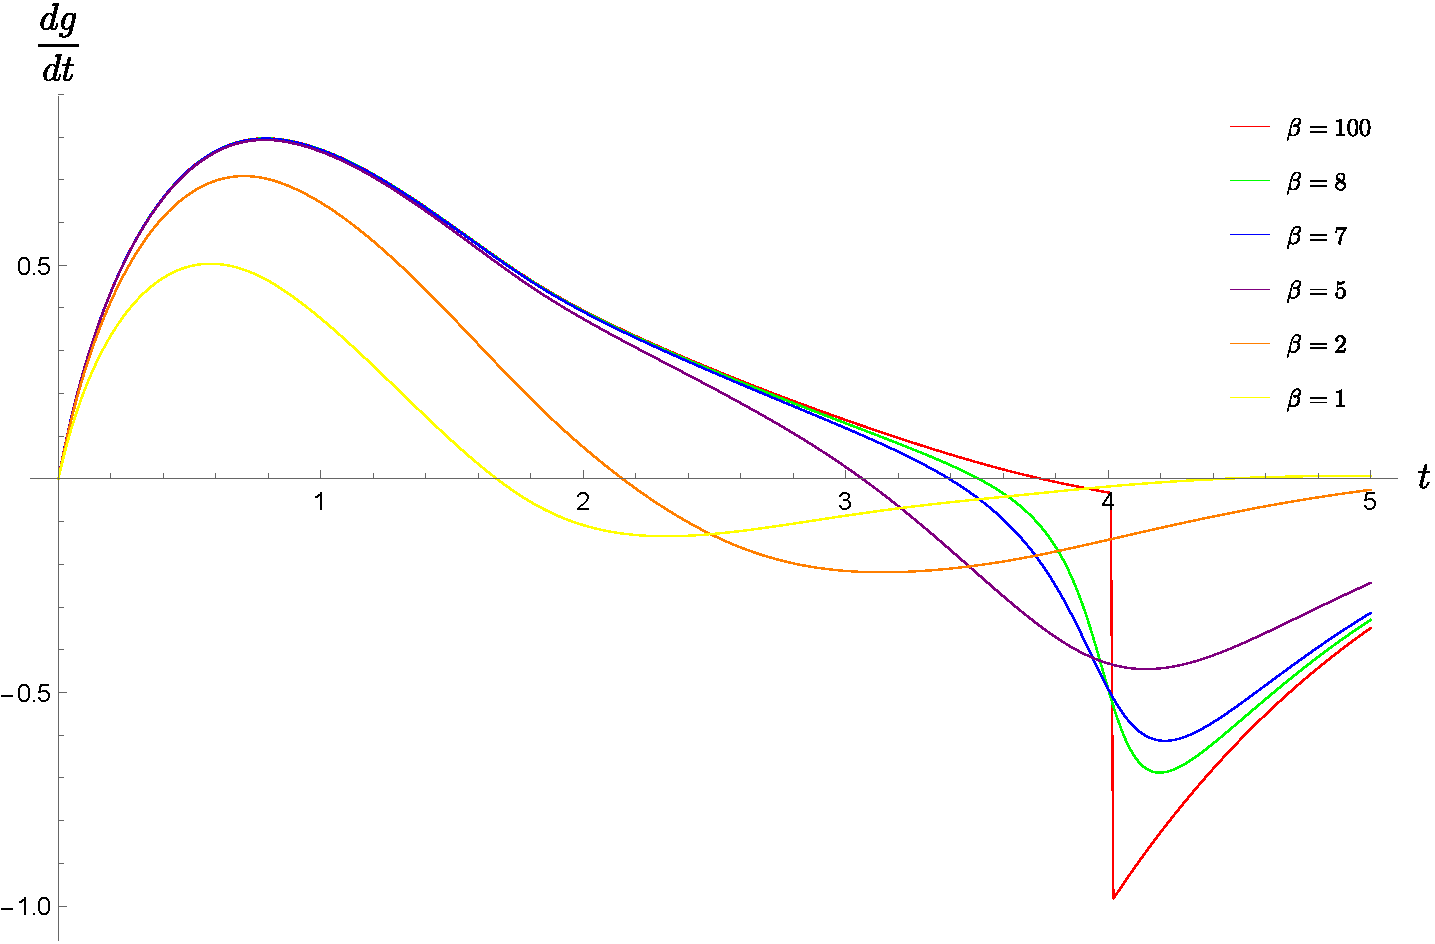
\includegraphics[scale=0.3]{MDM_trivial_L_topo_-1.pdf}
    \caption{The time derivative of the rate function, $dg/dt$, as a function of time for different values of the inverse temperature. We quench the system from a trivial to a topological regime (Regimes from I to II and from IV to III).}\end{center}
    \label{fig:MDM-trivial-L-topo--1}
    \end{figure}

\begin{figure}[h]   
\begin{center} 
    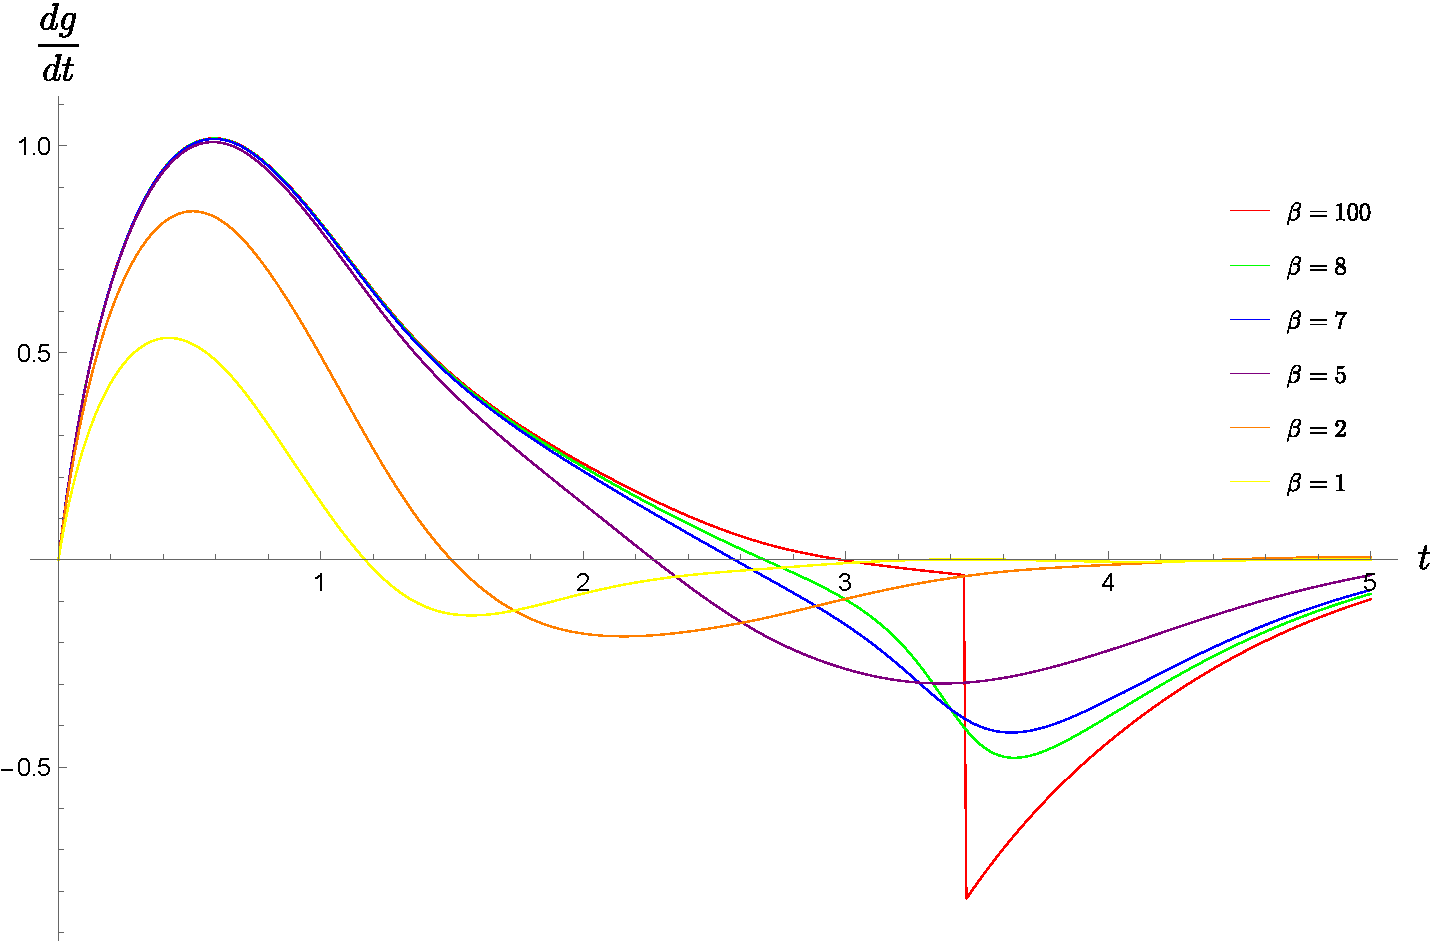
\includegraphics[scale=0.3]{MDM_topo_-1_trivial_L.pdf}
    \caption{The time derivative of the rate function, $dg/dt$, as a function of time for different values of the inverse temperature. The quench is from a topological to a trivial regime (Regimes from II to I and from III to IV).}\end{center}
     \label{fig:MDM-topo--1-trivial-L}
    \end{figure}

\begin{figure}[h]    
\begin{center}
    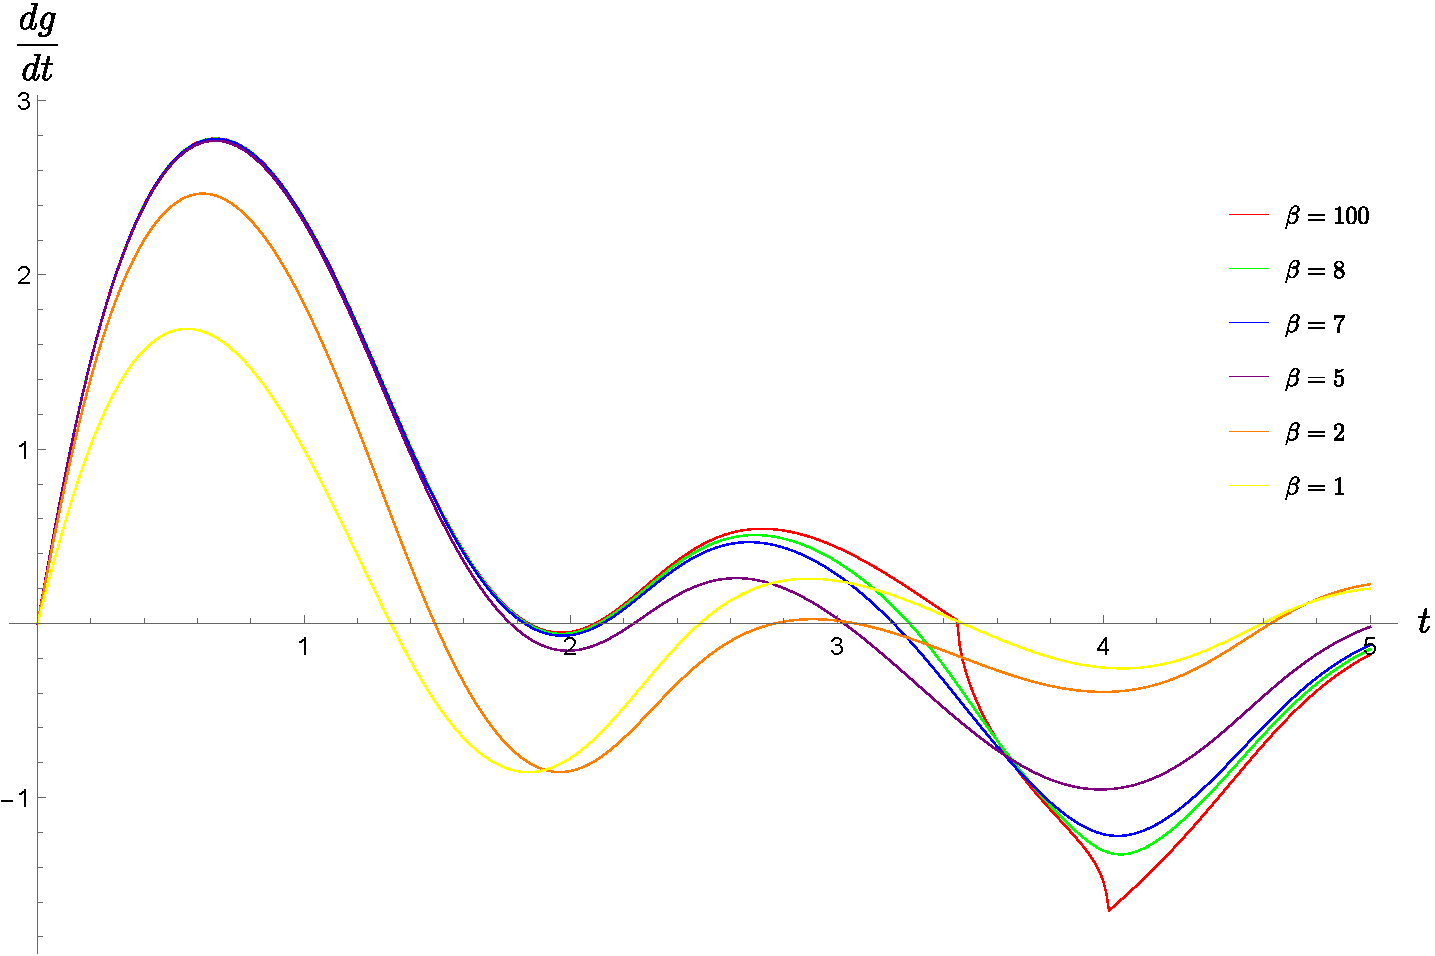
\includegraphics[scale=0.3]{MDM_topo_+1_topo_-1.pdf}
    \caption{The time derivative of the rate function, $dg/dt$, as a function of time for different inverse temperatures. The quantum quench is from a topological to a topological regime (Regimes from II to III and vice versa).}\end{center}
    \label{fig:MDM-topo-+1-topo--1}

\end{figure}


We observe that at zero temperature  there exist non-analyticities at the critical times -- the signatures of DQPTs. As we increase the temperature, these non-analyticities are gradually smeared out, resulting in smooth curves for higher finite temperatures. We note that the peak of the derivative $dg(t)/dt$ is drifted when increasing the temperature, in analogy to the usual drift of static quantum PTs at finite temperature~\cite{kem:que:smi:16}.


Next, we proceed by considering the cases in which we cross two PT points, as shown in Figures~6.7 and~6.8. At zero temperature we obtain a non-analytic behaviour, which gradually disappears for higher temperatures.


Finally, we have also studied the case in which we move inside the same topological regime from left to right and vice versa. We obtained smooth curves without non-analyticities, which we omit for the sake of briefness.


\begin{figure}[h!]
\begin{center}
    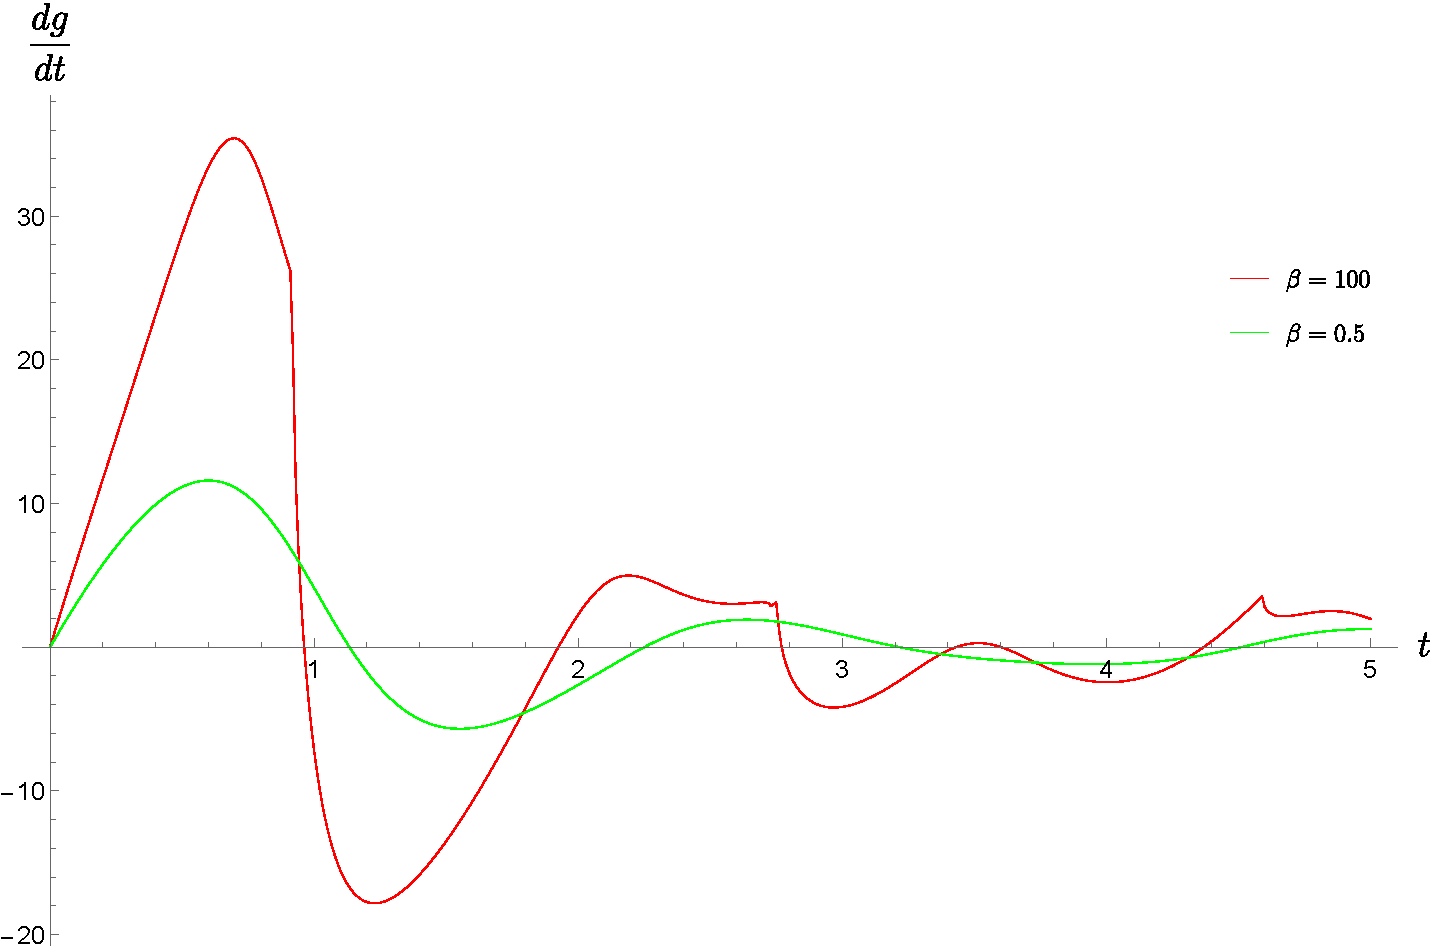
\includegraphics[scale=0.3]{MDM_trivial_L_topo_+1.pdf}
    
    \caption{The time derivative of the rate function, $dg/dt$, as a function of time for different values of the inverse temperature, in the case that we quench the system from a trivial to a topological regime (Regimes from I to III and from IV to II).}
    \end{center}
\label{fig:MDM-trivial-L-topo-+1}
\end{figure}  

\begin{figure}[h]
\begin{center}
    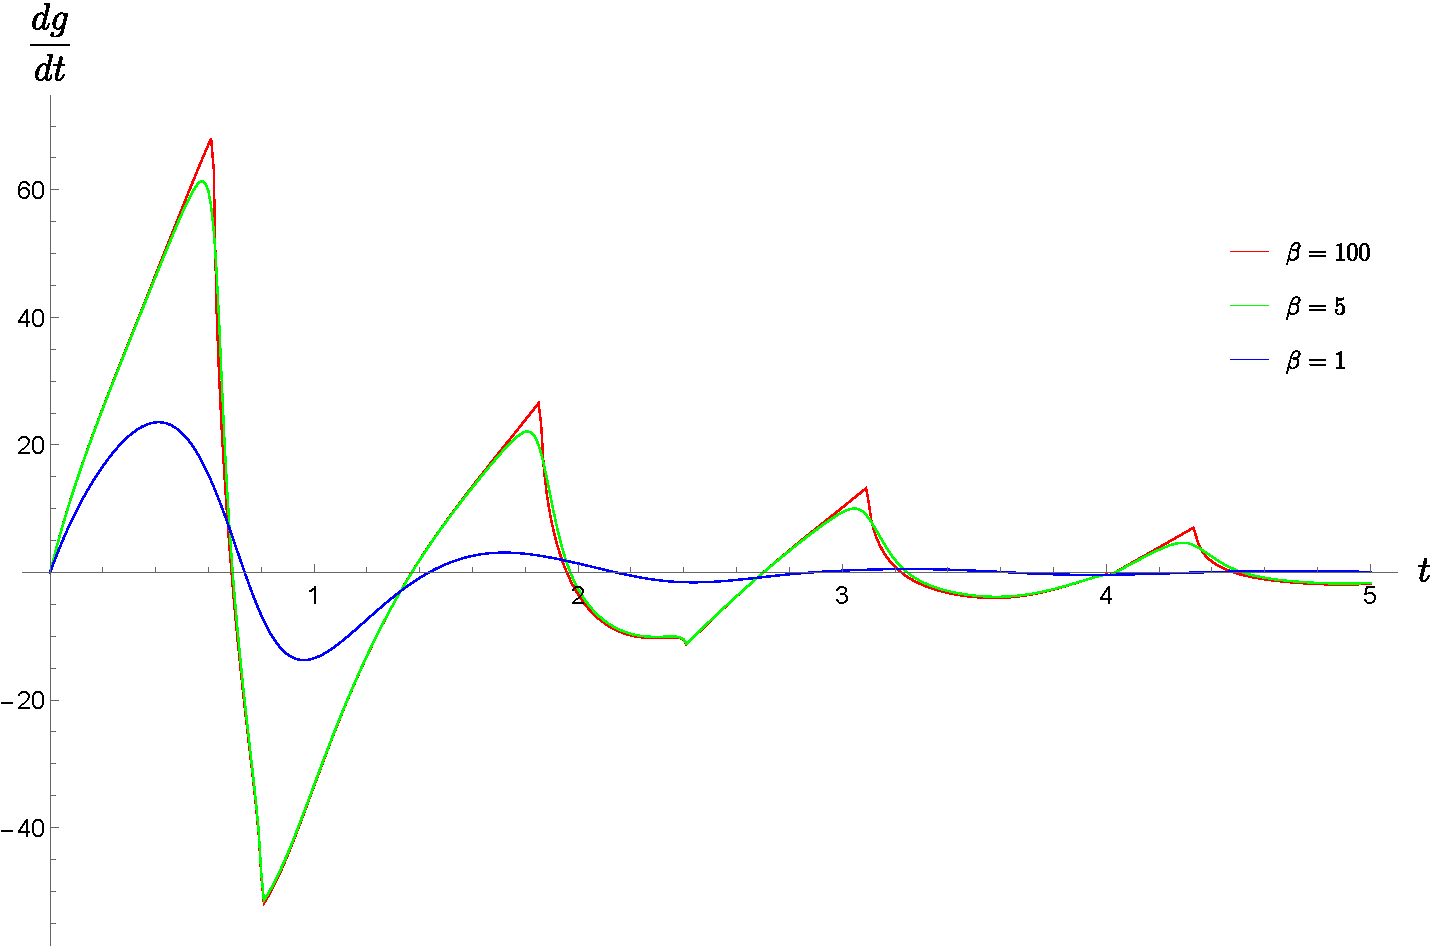
\includegraphics[scale=0.3]{MDM_topo_-1_trivial_R.pdf}
    \caption{The time derivative of the rate function, $dg/dt$, as a function of time for different values of the inverse temperature. The system is quenched from a topological to a trivial regime (Regimes from III to I and from II to IV).}\end{center}
\label{fig:MDM-topo--1-trivial-R}
\end{figure}





\section{Conclusions}

In this chapter, we analysed the fidelity and the interferometric generalisations of the LE for general mixed states, and applied them to the study of finite temperature DPTs in topological systems.
We showed that the dynamical fidelity susceptibility is the pullback of the Bures metric in the \emph{space of density matrices} (i.e., in the space of quantum states). On the other hand, the dynamical interferometric susceptibility is the pullback of a metric in the \emph{space of unitaries} (i.e., quantum channels). 
The difference between the two metrics reflects the fact that the fidelity is a measure of the state distinguishability between two {\em given} states $\rho$ and $\sigma$ in terms of observations, while the ``interferometric distinguishability'' quantifies how a quantum channel (a unitary $U$) changes an {\em arbitrary} state $\rho$ to $U \rho U^{\dagger}$. 
Therefore, while the ``interferometric distinguishability'' is in general more sensitive, and thus appropriate for the study of genuine (microscopic) systems, it is the fidelity that is the most suitable for the study of many-body system phases.
Moreover, interferometric experiments involve coherent superpositions of two states, which for many-body systems would require creating and manipulating genuine Schr\"{o}dinger cat-like states. This seems to be experimentally beyond current technology.

We analytically derived and presented closed expressions for the dynamical susceptibilities in the case of two-band Hamiltonians. At finite temperature, the fidelity LE indicates gradual disappearance of the zero-temperature DQPTs, while the interferometric LE predicts finite-temperature DPTs. We  applied this finite-temperature study on two representatives of TIs: the 1D SSH model and the 2D MD model. In perfect agreement with the general result, the fidelity-induced first derivatives are gradually smeared out with temperature, not exhibiting any critical behaviour at finite temperatures. This is also consistent with the study of 1D symmetry protected topological phases at finite temperatures that we presented in the previous two chapters. On the contrary, the interferometric LE exhibits critical behaviour even at finite temperatures (confirming previous studies on DPTs~\cite{hey:bud:17, bah:ban:dut:17}).
%
%\bibliographystyle{unsrt}
%\bibliography{bibforthesis}
%
%
%
%\end{document}
